\documentclass{standalone}
\usepackage{tikz}
\usetikzlibrary{patterns, positioning}


\begin{document}
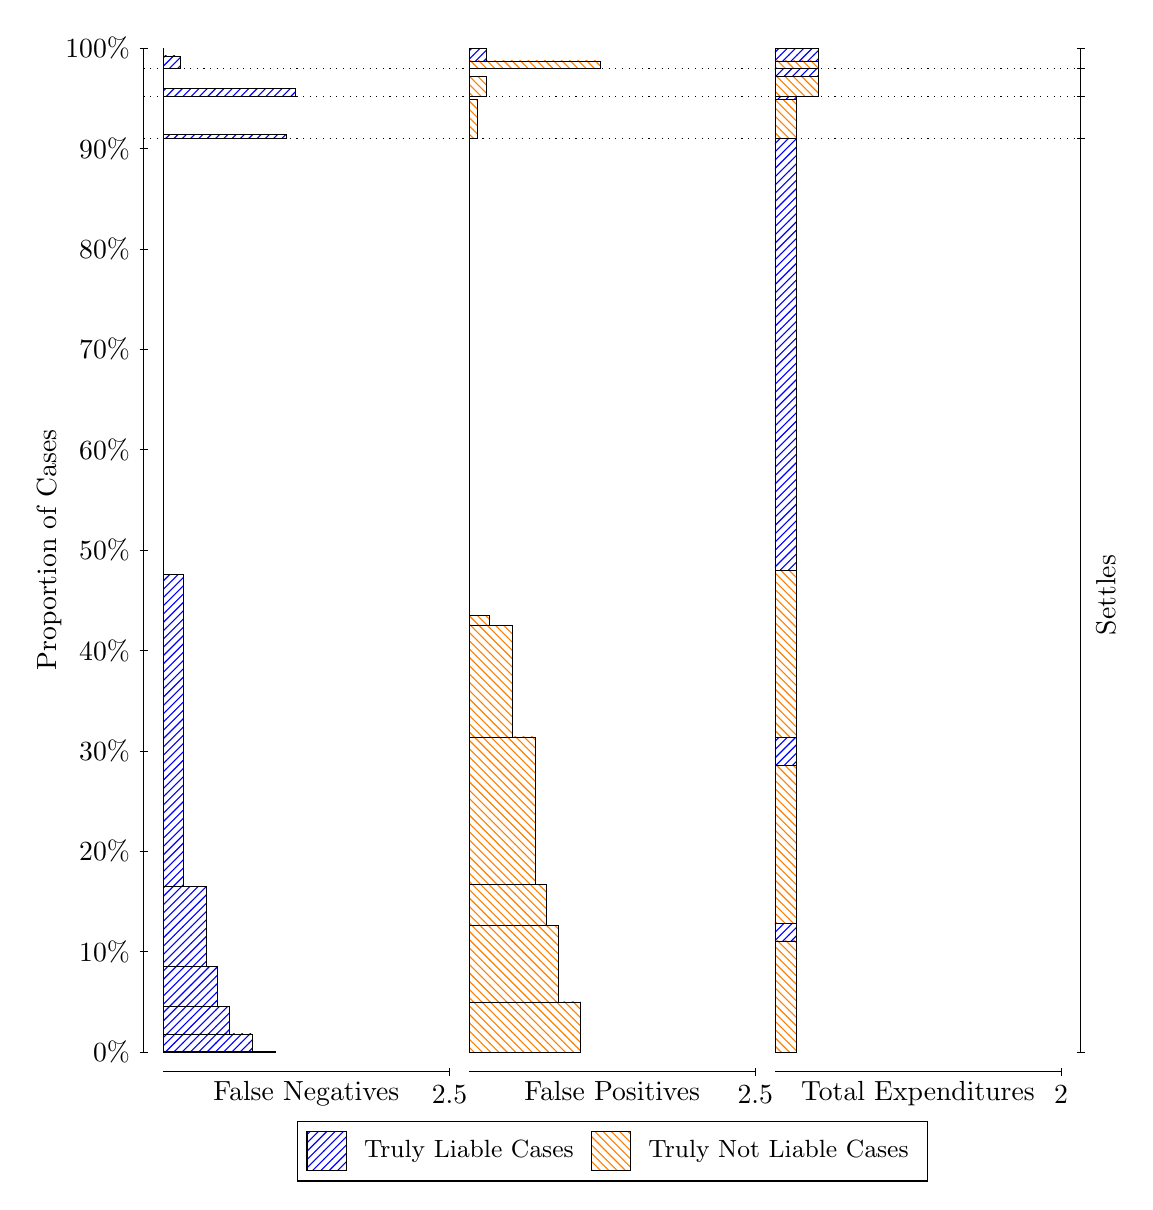
\begin{tikzpicture}
\draw[black, very thin] (1.5,1.75) -- (1.5,14.5);
\node[rotate=90, text=black, anchor=center] at (0.3, 8.125) {Proportion of Cases};
\draw[black, very thin] (1.45,1.75) -- (1.55,1.75);
\node[text=black, anchor=east] at (1.45, 1.75) {0\%};
\draw[black, very thin] (1.45,3.025) -- (1.55,3.025);
\node[text=black, anchor=east] at (1.45, 3.025) {10\%};
\draw[black, very thin] (1.45,4.3) -- (1.55,4.3);
\node[text=black, anchor=east] at (1.45, 4.3) {20\%};
\draw[black, very thin] (1.45,5.575) -- (1.55,5.575);
\node[text=black, anchor=east] at (1.45, 5.575) {30\%};
\draw[black, very thin] (1.45,6.85) -- (1.55,6.85);
\node[text=black, anchor=east] at (1.45, 6.85) {40\%};
\draw[black, very thin] (1.45,8.125) -- (1.55,8.125);
\node[text=black, anchor=east] at (1.45, 8.125) {50\%};
\draw[black, very thin] (1.45,9.4) -- (1.55,9.4);
\node[text=black, anchor=east] at (1.45, 9.4) {60\%};
\draw[black, very thin] (1.45,10.675) -- (1.55,10.675);
\node[text=black, anchor=east] at (1.45, 10.675) {70\%};
\draw[black, very thin] (1.45,11.95) -- (1.55,11.95);
\node[text=black, anchor=east] at (1.45, 11.95) {80\%};
\draw[black, very thin] (1.45,13.225) -- (1.55,13.225);
\node[text=black, anchor=east] at (1.45, 13.225) {90\%};
\draw[black, very thin] (1.45,14.5) -- (1.55,14.5);
\node[text=black, anchor=east] at (1.45, 14.5) {100\%};

\draw[black, very thin] (13.4,1.75) -- (13.4,14.5);
\draw[black, very thin] (13.35,1.75) -- (13.45,1.75);
\node[anchor=west] at (13.35, 1.75) {};
\draw[black, very thin] (13.35,13.356) -- (13.45,13.356);
\node[anchor=west] at (13.35, 13.356) {};
\draw[black, very thin] (13.35,13.89) -- (13.45,13.89);
\node[anchor=west] at (13.35, 13.89) {};
\draw[black, very thin] (13.35,14.237) -- (13.45,14.237);
\node[anchor=west] at (13.35, 14.237) {};
\draw[black, very thin] (13.35,14.5) -- (13.45,14.5);
\node[anchor=west] at (13.35, 14.5) {};

\draw[black, very thin, pattern color=blue, pattern=north east lines] (1.75,1.75) rectangle (3.167,1.7589);
\draw[black, very thin, pattern color=blue, pattern=north east lines] (1.75,1.7589) rectangle (2.8763,1.9803);
\draw[black, very thin, pattern color=blue, pattern=north east lines] (1.75,1.9803) rectangle (2.5857,2.327);
\draw[black, very thin, pattern color=blue, pattern=north east lines] (1.75,2.327) rectangle (2.4403,2.8383);
\draw[black, very thin, pattern color=blue, pattern=north east lines] (1.75,2.8383) rectangle (2.295,3.8486);
\draw[black, very thin, pattern color=blue, pattern=north east lines] (1.75,3.8486) rectangle (2.0043,7.8152);
\draw[black, very thin, pattern color=orange, pattern=north west lines] (1.75,7.8152) rectangle (1.75,13.356);
\draw[black, very thin, pattern color=blue, pattern=north east lines] (1.75,13.356) rectangle (3.3123,13.402);
\draw[black, very thin, pattern color=orange, pattern=north west lines] (1.75,13.402) rectangle (1.75,13.89);
\draw[black, very thin, pattern color=blue, pattern=north east lines] (1.75,13.89) rectangle (3.4213,13.99);
\draw[black, very thin, pattern color=orange, pattern=north west lines] (1.75,13.99) rectangle (1.75,14.237);
\draw[black, very thin, pattern color=blue, pattern=north east lines] (1.75,14.237) rectangle (1.968,14.4);
\draw[black, very thin, pattern color=orange, pattern=north west lines] (1.75,14.4) rectangle (1.75,14.5);
\draw[black, very thin, pattern color=orange, pattern=north west lines] (5.6333,1.75) rectangle (7.0503,2.3852);
\draw[black, very thin, pattern color=orange, pattern=north west lines] (5.6333,2.3852) rectangle (6.7597,3.3623);
\draw[black, very thin, pattern color=orange, pattern=north west lines] (5.6333,3.3623) rectangle (6.6143,3.8736);
\draw[black, very thin, pattern color=orange, pattern=north west lines] (5.6333,3.8736) rectangle (6.469,5.7518);
\draw[black, very thin, pattern color=orange, pattern=north west lines] (5.6333,5.7518) rectangle (6.1783,7.1628);
\draw[black, very thin, pattern color=orange, pattern=north west lines] (5.6333,7.1628) rectangle (5.8877,7.2907);
\draw[black, very thin, pattern color=blue, pattern=north east lines] (5.6333,7.2907) rectangle (5.6333,13.356);
\draw[black, very thin, pattern color=orange, pattern=north west lines] (5.6333,13.356) rectangle (5.7423,13.844);
\draw[black, very thin, pattern color=blue, pattern=north east lines] (5.6333,13.844) rectangle (5.6333,13.89);
\draw[black, very thin, pattern color=orange, pattern=north west lines] (5.6333,13.89) rectangle (5.8513,14.136);
\draw[black, very thin, pattern color=blue, pattern=north east lines] (5.6333,14.136) rectangle (5.6333,14.237);
\draw[black, very thin, pattern color=orange, pattern=north west lines] (5.6333,14.237) rectangle (7.3047,14.336);
\draw[black, very thin, pattern color=blue, pattern=north east lines] (5.6333,14.336) rectangle (5.8513,14.5);
\draw[black, very thin, pattern color=orange, pattern=north west lines] (9.5167,1.75) rectangle (9.7892,3.161);
\draw[black, very thin, pattern color=blue, pattern=north east lines] (9.5167,3.161) rectangle (9.7892,3.3823);
\draw[black, very thin, pattern color=orange, pattern=north west lines] (9.5167,3.3823) rectangle (9.7892,5.3884);
\draw[black, very thin, pattern color=blue, pattern=north east lines] (9.5167,5.3884) rectangle (9.7892,5.7441);
\draw[black, very thin, pattern color=orange, pattern=north west lines] (9.5167,5.7441) rectangle (9.7892,7.8677);
\draw[black, very thin, pattern color=blue, pattern=north east lines] (9.5167,7.8677) rectangle (9.7892,13.356);
\draw[black, very thin, pattern color=orange, pattern=north west lines] (9.5167,13.356) rectangle (9.7892,13.844);
\draw[black, very thin, pattern color=blue, pattern=north east lines] (9.5167,13.844) rectangle (9.7892,13.89);
\draw[black, very thin, pattern color=orange, pattern=north west lines] (9.5167,13.89) rectangle (10.062,14.136);
\draw[black, very thin, pattern color=blue, pattern=north east lines] (9.5167,14.136) rectangle (10.062,14.237);
\draw[black, very thin, pattern color=orange, pattern=north west lines] (9.5167,14.237) rectangle (10.062,14.336);
\draw[black, very thin, pattern color=blue, pattern=north east lines] (9.5167,14.336) rectangle (10.062,14.5);
\draw[black, dotted] (1.5,13.356) -- (13.4,13.356);
\draw[black, dotted] (1.5,13.89) -- (13.4,13.89);
\draw[black, dotted] (1.5,14.237) -- (13.4,14.237);
\draw[black, very thin] (1.75,1.5) -- (5.3833,1.5);
\node[text=black, anchor=north] at (3.5667, 1.5) {False Negatives};
\draw[black, very thin] (5.3833,1.45) -- (5.3833,1.55);
\node[text=black, anchor=north] at (5.3833, 1.45) {2.5};

\draw[black, very thin] (5.6333,1.5) -- (9.2667,1.5);
\node[text=black, anchor=north] at (7.45, 1.5) {False Positives};
\draw[black, very thin] (9.2667,1.45) -- (9.2667,1.55);
\node[text=black, anchor=north] at (9.2667, 1.45) {2.5};

\draw[black, very thin] (9.5167,1.5) -- (13.15,1.5);
\node[text=black, anchor=north] at (11.333, 1.5) {Total Expenditures};
\draw[black, very thin] (13.15,1.45) -- (13.15,1.55);
\node[text=black, anchor=north] at (13.15, 1.45) {2};

\node[text=black, centered, rotate=90] at (13.72, 7.5529) {Settles};




\draw (7.449999999999999,1.5) node[draw=none] (baseCoordinate) {};
\begin{scope}[align=center]
        \matrix[scale=0.5, draw=black, below=0.5cm of baseCoordinate, nodes={draw}, column sep=0.1cm]{
            \node[rectangle, draw, minimum width=0.5cm, minimum height=0.5cm, pattern color=blue, pattern=north east lines] {}; &
            \node[draw=none, font=\small, text=black] (B) {Truly Liable Cases}; &
            \node[rectangle, draw, minimum width=0.5cm, minimum height=0.5cm, pattern color=orange, pattern=north west lines] {}; &
            \node[draw=none, font=\small, text=black] (B) {Truly Not Liable Cases}; \\
            };
\end{scope}

\end{tikzpicture}
\end{document}